On modélise un passage de spectacle de voltige aérienne en duo de la manière suivante :

\begin{itemize}[label=$\bullet$]
\item on se place dans un repère orthonormé \Oijk, une unité représentant un mètre;

\item l'avion n\up{o} 1 doit relier le point O au point $\mathrm{A}(0~;~200~;~0)$ selon une trajectoire rectiligne, à la vitesse constante de $\np[m/s]{200}$;

\item l'avion n\up{o} 2 doit, quant à lui, relier le point $\mathrm{B}(-33~;~75~;~44)$ au point $\mathrm{C}(87~;~75~;~-116)$ également selon une trajectoire rectiligne, et à la vitesse constante de $\np[m/s]{200}$.

\item au même instant, l'avion \no 1 est au point O et l'avion \no 2 est au point B.
\end{itemize}
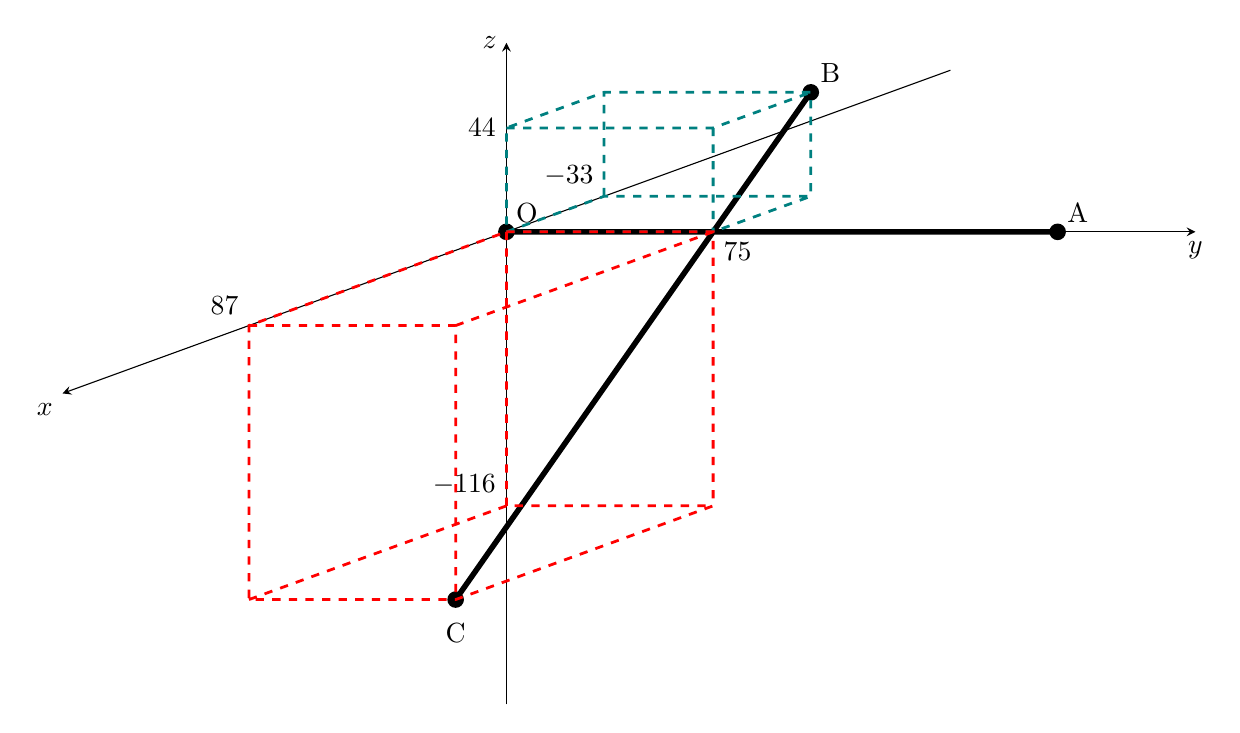
\begin{tikzpicture}[x={(-160:0.4mm)},y={(0:0.35mm)},z={(90:0.3mm)},>=stealth]
	\draw[->] (-150,0,0) -- (150,0,0) node[below left]{$x$};
	\draw[->] (0,0,0) -- (0,250,0) node[below]{$y$};
	\draw[->] (0,0,-200) -- (0,0,80) node[left]{$z$};
	\fill (0,0,0) circle (3pt) node[above right]{O};
	\fill (0,200,0) circle (3pt) node[above right]{A};
	\fill (87,75,-116) circle (3pt) node[below=5pt]{C};
	\fill (-33,75,44) circle (3pt) node[above right]{B};
	\draw[line width=2pt] (0,0,0) -- (0,200,0) (87,75,-116) -- (-33,75,44) ;
	\draw[teal,dashed,line width=1pt] (0,0,0) -- (0,75,0) node[color=black,below right]{75} -- (-33,75,0) -- (-33,75,44) -- (-33,0,44) -- (0,0,44)node[black,left]{44} -- cycle
	(0,0,44) -- (0,75,44) -- (-33,75,44) (0,75,44) -- (0,75,0)
	(0,0,0) -- (-33,0,0)node[black,above left]{$-33$} -- (-33,75,0) (-33,0,0) -- (-33,0,44);
	\draw[red,dashed,line width=1pt] (0,0,0) -- (0,75,0) -- (0,75,-116) -- (87,75,-116) -- (87,0,-116) -- (87,0,0)node[black,above left]{87} -- cycle
	(87,0,0)--(87,75,0) -- (87,75,-116) (87,75,0) -- (0,75,0)
	(0,0,0) -- (0,0,-116)	(87,0,-116) -- (0,0,-116)node[black, above left]{$-116$} --(0,75,-116);
\end{tikzpicture}
\begin{enumerate}
\item Justifier que l'avion \no 2 mettra autant de temps à parcourir le segment [BC] que l'avion \no 1 à parcourir le segment [OA].
\item Montrer que les trajectoires des deux avions se coupent.
\item Les deux avions risquent-ils de se percuter lors de ce passage ?
\end{enumerate}
